\documentclass[a4paper,12pt,french]{article}
\usepackage[T1]{fontenc}
\usepackage[utf8]{inputenc}
\usepackage{graphicx}
\usepackage{calc}

\usepackage[french]{babel}

\usepackage{siunitx}
\usepackage{amssymb}

\newcommand{\e}[1]{\vspace{5mm}\noindent \textbf{\underline{#1}}}

\newcommand{\makeline}{\noindent\makebox[\linewidth]{\rule{\linewidth}{0.4pt}}} 

\setcounter{secnumdepth}{-1}

\begin{document}

\section{Exercice 1}

On considère une source monochromatique de longueur d'onde $\lambda = \SI{600}{\nano\meter}$ éclairant un interféromètre de Michelson d'épaisseur $e$. À la sortie du dispositif, on place une lentille convergente de distance focale $f'=\SI{50}{\centi\meter}$.

\begin{enumerate}
	\item Dans quelle configuration doit on placer le Michelson pour observer des anneaux d'interférence ? Tracer alors le dispositif permettant l'observation des franges.
	\item Déterminer la différence de marche entre deux rayons interférant sur l'écran.
	\item Exprimer le rayon des anneaux en fonction de l'ordre d'interférence $p$, de $\lambda$ et de $f'$.
	\item Quel anneau présente un ordre d'interférence maximal ? Le calculer.
	\item L'image ci-dessous représente la figure d'interférences obtenue (les traits noirs correspondent aux maxima d'intensité). Calculer l'épaisseur $e$ de la lame d'air. Commentaire.
\end{enumerate}

\begin{figure}[h]
	\centering
	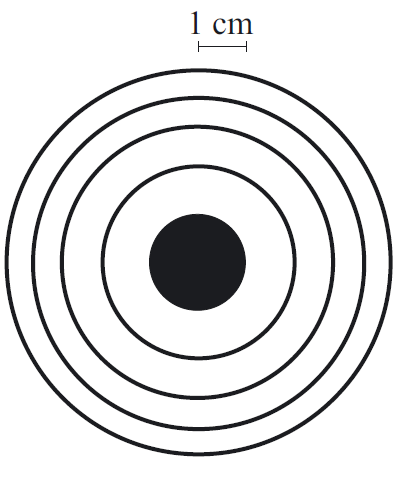
\includegraphics[width=.6\textwidth]{ex_01.png}
\end{figure}

\newpage

\section{Exercice 2}

On considère un dispositif de rails de Laplace classique, mais la barre glissant sans frottement sur les rails est attachée en $M$ à un ressort de longueur à vide $l_0$ et de raideur $k$. On note $A$ le point d'attache fixe du ressort à l'autre extrémité. L'ensemble est plongé dans un champ magnétique permanent et uniforme $\vec{B}$. Le circuit a une résistance $R$, la tige de masse $m$ a une longueur $a$. À l'instant $t=0$, on déplace la tige initialement au repos à l'abscisse $x=0$ jusqu'à l'abscisse $x_0>0$ et on lâche sans vitesse initiale.

\begin{figure}[h]
	\centering
	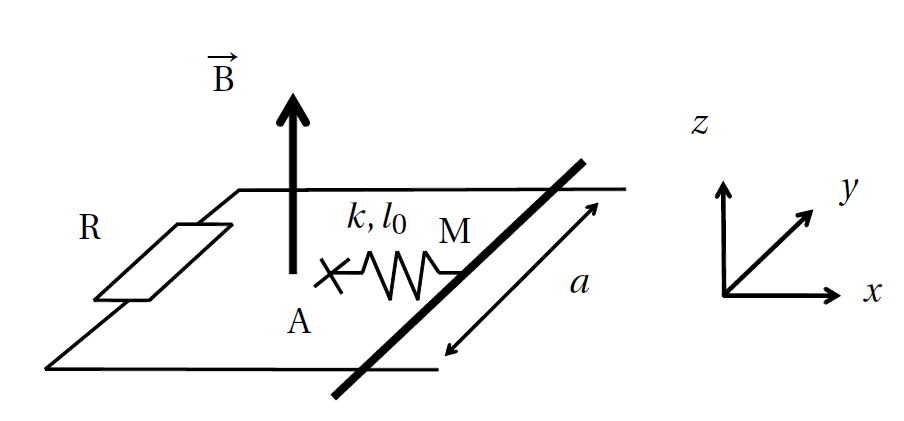
\includegraphics[width=.7\textwidth]{ex_02.png}
\end{figure}

\begin{enumerate}
	\item Décrire qualitativement l'évolution du système.
	\item Donner le sens réel $i$ du courant induit selon le sens de déplacement de la barre.
	\item Mettre l'équation du mouvement sous la forme $\ddot{x}+\frac{1}{\tau}\dot{x}+\omega_0^2x = 0$.
	\item Quelle est la condition pour avoir un régime pseudopériodique ? Commenter cette expression.
	\item Donner l'expression de $x(t)$ dans ce cas.
	\item Effectuer un bilan d'énergie et le commenter. Au cours de l'expérience, quelle est la quantité totale d'énergie dissipée dans la résistance ? 
\end{enumerate}

\newpage

\begin{scriptsize}
	
\e{Nom :} \hfill \e{Date :} \hspace{3cm}

\begin{center}
\begin{tabular}{|p{.1\textwidth}|p{.8\textwidth}|p{.1\textwidth}|}
	\hline
	& \textbf{Compréhension et application du cours (4 points)} & \\ \hline
	0/4 & Notions mal connues ou mélangées. Définitions, lois ou relations fondamentales non sues ou mal énoncées. & \\ \hline
	1/4 & Connaissances fragmentaires. Notions mal comprises ou utilisées à contre-sens. Difficultés à appliquer des lois. & \\ \hline
	2/4 & Cours globalement su mais difficultés à l'appliquer ou trop d'imprécisions dans les énoncés. & \\ \hline
	3/4 & Cours plutôt bien énoncé et appliqué mais quelques imprécisions sur des points classiques. & \\ \hline
	4/4 & Cours connu, énoncé avec précision et appliqué avec rigueur. & \\ \hline
	
	& \textbf{Calculs littéraux et numériques (2 points)} & \\ \hline
	0/2 & Trop d'erreurs de calcul ou d'applications numériques. & \\ \hline
	1/2 & Quelques erreurs. & \\ \hline
	2/2 & Calculs bien menés ou corrigés en autonomie. & \\ \hline
	
	& \textbf{Démarche scientifique (3 points)} & \\ \hline
	0/3 & Démarche désorganisée, sans stratégie apparente ou incohérente avec l'énoncé. & \\ \hline
	1/3 & Tentative de stratégie mais manquant de rigueur ou mal adaptée au problème. & \\ \hline
	2/3 & Démarche globalement logique et structurée mais quelques étapes floues ou peu justifiées. & \\ \hline
	3/3 & Démarche claire, logique et rigoureuse. & \\ \hline
	
	& \textbf{Esprit critique et vérification des résultats (3 points)} & \\ \hline
	0/3 & Les résultats ne sont pas critiqués a posteriori & \\ \hline
	1/3 & Efforts faits, mais l'utilisation de l'homogénéité, de l'interprétation physique et de la comparaison à des valeurs ou expressions connues reste anecdotique. & \\ \hline
	2/3 & Démarche critique mais quelques erreurs non corrigées ou interprétations de certains résultats peu convaincantes. & \\ \hline
	3/3 & Démarche critique systématique permettant de corriger certaines erreurs en autonomie ou d'apporter un éclaircissement scientifique sur certains résultats. & \\ \hline
	
	& \textbf{Expression orale (2 points)} & \\ \hline
	0/2 & Expression confuse, vocabulaire inadapté, fautes répétées d'expression. & \\ \hline
	1/2 & Expression compréhensible mais parfois imprécise ou peu fluide & \\ \hline
	2/2 & Expression claire, structurée et précise. Vocabulaire scientifique. & \\ \hline
	
	& \textbf{Expression écrite (2 points)} & \\ \hline
	0/2 & Tableau mal tenu, absence de figures, notations incorrectes ou dessins inutilisables. & \\ \hline
	1/2 & Tableau soigné mais les schémas manquent de lisibilité ou de pertinence. & \\ \hline
	2/2 & Tableau soigné. Schémas clairs, bien annotés, exploités dans l'argumentation. & \\ \hline
	
	& \textbf{Réactivité aux questions et indications (2 points)} & \\ \hline
	0/2 & Incapacité à comprendre les questions ou à s'adapter aux remarques. & \\ \hline
	1/2 & Compréhension partielle ou tardive, adaptation laborieuse. & \\ \hline
	2/2 & Bonne écoute, réponses adaptées et correction rapide d'éventuelles erreurs. & \\ \hline
	
	& \textbf{Autonomie et initiative (2 points)} & \\ \hline
	0/2 & Attend systématiquement des indications pour avancer. & \\ \hline
	1/2 & Quelques initiatives mais peu pertinentes ou timides. & \\ \hline
	2/2 & Prend des initiatives réfléchies, explore différentes pistes avec jugement. & \\ \hline
	
	& \textbf{Total (20 points)} & \\
	& & \\ \hline
\end{tabular} 
\end{center}
\end{scriptsize}

\end{document}